% Misión 7: la estación de carga. Portada y vuelo paso a paso.
% NED (este, norte): patrulla a 8 m por la cerca, de (E -31, N -2) a (E -31, N 42) a (E 31, N 42) a
% (E 31, N -2). La estación real (ArUco 42) está en E 18, N 30; "el mapa" dice E 19.5 (1.5 m de error).

\begin{frame}{Misión 7: la estación de carga}
  \begin{columns}[c]
    \column{0.56\textwidth}
    \begin{tikzpicture}
      \node[inner sep=0] (im) {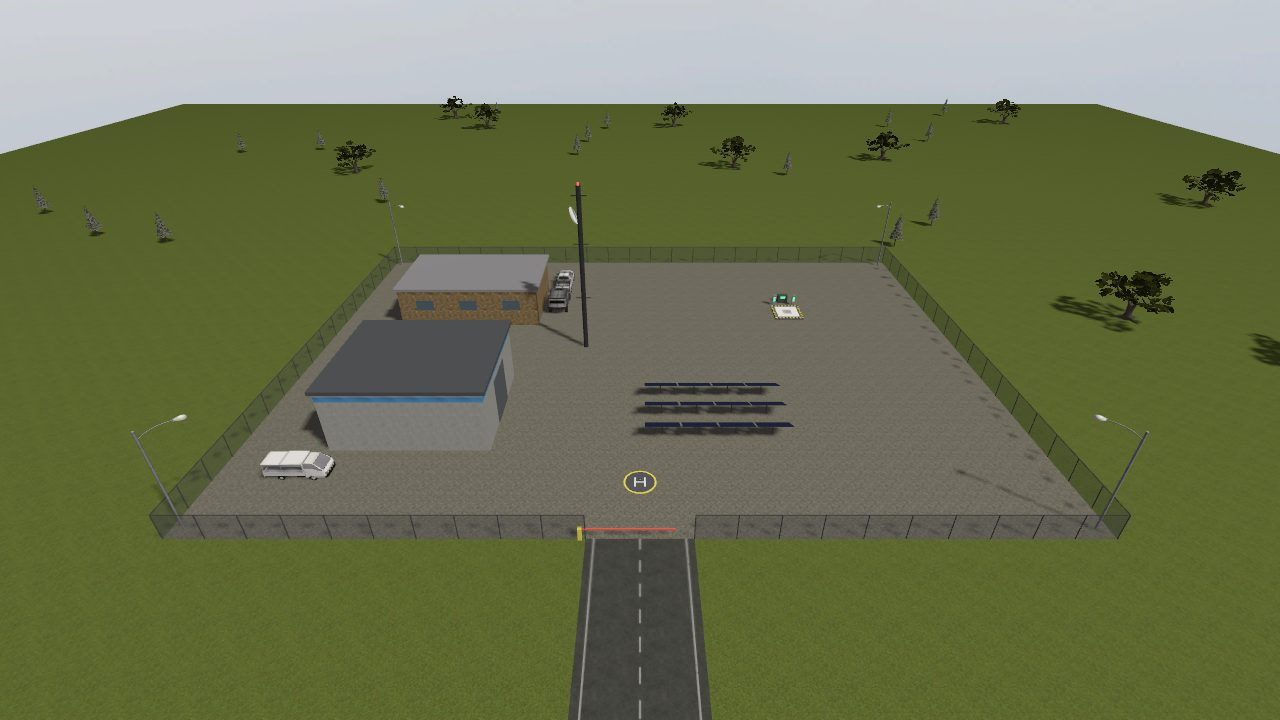
\includegraphics[width=\linewidth]{base_carga}};
      \node[anchor=north west,fill=azul,text=white,font=\bfseries\scriptsize,rounded corners=2pt]
        at ([xshift=4pt,yshift=-4pt]im.north west) {MISIÓN 7 · NIVEL 3 \nivel{3}};
    \end{tikzpicture}\\[0.3em]
    \small\textbf{Escenario}: un dron de vigilancia patrulla la cerca de una base. Con batería baja va a su
    estación, \textbf{aterriza con precisión} sobre el ArUco 42, ``carga'' y \textbf{regresa a patrullar justo
    donde se quedó}.
    \column{0.41\textwidth}
    \ficha{x500_cam_abajo}{x500\_cam\_abajo}{base\_carga}{estacion\_carga + detector\_aruco}%
      {\cmd{battery\_monitor} y \cmd{square\_mission}}{aterrizaje de precisión con la cámara}%
      {cada carga a \textless 0.3 m del centro del ArUco}
  \end{columns}
\end{frame}

\begin{frame}{La estación, paso a paso}
  \begin{columns}[c]
    \column{0.44\textwidth}\centering
    \begin{tikzpicture}[x=0.075cm,y=0.075cm]
      \draw[gray!50,fill=gray!8] (-36,-7) rectangle (36,47);
      \fill[gray!55] (-27,4) rectangle (-13,16); \node[font=\tiny] at (-20,10) {hangar};
      \draw[azul!35,thick] (-31,-2) rectangle (31,42);
      \node[draw,circle,fill=azulclaro,inner sep=0.3pt,font=\tiny] at (0,0) {H};
      \fill[orange] (16.3,28.3) rectangle (19.7,31.7);
      \node[font=\tiny,below] at (18,28) {estación};
      % por dónde va
      \draw[azul,line width=1.5pt,visible on=<1>] (-31,-2) -- (-31,30);
      \draw[azul,line width=1.5pt,visible on=<2->] (-31,-2) -- (-31,42) -- (-5,42);
      \draw[naranja,dashed,thick,-{Stealth},visible on=<3>] (-4,41) -- (17.5,31);
      \draw[naranja,dashed,thick,-{Stealth},visible on=<6>] (17,32) -- (-4,41);
      \draw[azul,line width=1.5pt,visible on=<7>] (-5,42) -- (31,42) -- (31,-2) -- (-31,-2);
      \node[font=\large,text=rojo,visible on=<2->] at (-5,42) {$\times$};
      \node[font=\tiny,text=rojo,above,visible on=<2->] at (-5,43.5) {aquí se quedó};
      \only<1>{\node at (-31,30) {\dronarriba{0.55cm}};}
      \only<2>{\node at (-5,42) {\dronarriba{0.55cm}};}
      \only<3>{\node at (19.5,30) {\dronarriba{0.55cm}};}
      \only<4-5>{\node at (18,30) {\dronarriba{0.55cm}};}
      \only<6>{\node at (-5,42) {\dronarriba{0.55cm}};}
      \only<7>{\node at (0,0) {\dronarriba{0.55cm}};}
    \end{tikzpicture}\\
    % la batería
    \begin{tikzpicture}
      \draw[rounded corners=1pt] (0,0) rectangle (3,0.35); \fill (3,0.1) rectangle (3.08,0.25);
      \only<1>{\fill[verde!70] (0.04,0.04) rectangle (2.7,0.31); \node[font=\tiny] at (1.5,0.175) {90 \%};}
      \only<2-4>{\fill[naranja] (0.04,0.04) rectangle (1.8,0.31); \node[font=\tiny] at (1.5,0.175) {60 \%};}
      \only<5>{\fill[verde!70] (0.04,0.04) rectangle (2.96,0.31); \node[font=\tiny] at (1.5,0.175) {100 \%};}
      \only<6-7>{\fill[verde!70] (0.04,0.04) rectangle (2.6,0.31); \node[font=\tiny] at (1.5,0.175) {85 \%};}
      \draw[rojo,thick] (1.8,-0.08) -- (1.8,0.43) node[above,font=\tiny,text=rojo] {low\_percent};
    \end{tikzpicture}
    \column{0.54\textwidth}
    \estados{1/PATROL,2-3/TO\_STATION,4/PRECISION,5/CHARGING,6/RESUME,7/PATROL}
    \vspace{0.3em}

    \only<1>{\begin{terminal}{ros2 launch x500\_retos estacion.launch.py}
Arriba. Patrullando\\
patrulla tramo 1, batería 90 \%
    \end{terminal}\small Recorre la cerca a 8 m. En SITL la batería baja \textbf{rapidísimo} armado (100 a 50 \% en
      30 s).}%
    \only<2>{\begin{terminal}{estacion\_carga}
Batería en 60 \%: dejo la patrulla en el tramo 2\\
\ \ y voy a cargar
    \end{terminal}\small Bajo \cmd{low\_percent}. Antes de irse \textbf{guarda dónde estaba} ({\color{rojo}$\times$}) y
      en qué tramo.}%
    \only<3>{\begin{terminal}{estacion\_carga}
Sobre la estación (según el mapa). ...
    \end{terminal}\small Llega por GPS a la estación \textbf{según el mapa}, que tiene 1.5 m de error a
      propósito.}%
    \only<4>{\begin{columns}[c]
      \column{0.42\linewidth}\centering
      \begin{tikzpicture}[scale=0.55]
        \fill[gray!40] (-1.7,0) rectangle (1.7,0.25); \fill[black] (-0.35,0.25) rectangle (0.35,0.3);
        \draw[azul,thick,-{Stealth}] (1.5,4) -- (0.1,3.3);
        \draw[verde,thick,-{Stealth}] (0,3.1) -- (0,0.9);
        \node[font=\tiny,text=gris] at (1.5,4.4) {el mapa};
        \draw[rojo,dashed] (-1.8,1.05) -- (1.8,1.05);
      \end{tikzpicture}
      \column{0.56\linewidth}\scriptsize
      \textbf{Tu TODO}: con lo que ve la cámara, \textbf{centrarse} sobre el ArUco 42 y bajar \textbf{solo si
      ya está centrado} (\textless 0.2 m). A 0.8 m, Land.
    \end{columns}
    \begin{terminal}{estacion\_carga}
bajando: 2.1 m sobre la plataforma, ...
    \end{terminal}}%
    \only<5>{\begin{terminal}{estacion\_carga}
En la estación, a 0.12 m del centro OK.\\
\ \ Cargando 5 s...
    \end{terminal}\small En SITL, \textbf{desarmar es cargar}: la batería vuelve a 100 \%.}%
    \only<6>{\begin{terminal}{estacion\_carga}
Regresando a patrullar desde donde me quedé\\
\ \ (norte 42.0, este -5.0)\\
De vuelta en la patrulla (tramo 2)
    \end{terminal}\small Vuelve a armar, despega y regresa \textbf{al punto guardado}, no al principio.}%
    \only<7>{\begin{terminal}{estacion\_carga}
Patrulla completa (1 vuelta/s). Regresando a casa\\
En casa y desarmado. Resultado:\\
\ \ carga 1: aterrizó a 0.12 m del centro\\
\ \ \ \ (máximo 0.3) OK\\
Misión cumplida
    \end{terminal}\credito{Números de ejemplo: dependen de tu TODO.}}%
  \end{columns}
\end{frame}
